\documentclass{article}
\usepackage[T1] {fontenc}
\usepackage[italian]{babel}
\usepackage{cite}

\usepackage{graphicx}
\graphicspath{ {./images/} }
\usepackage{float}

% Per i link nell'indice
\usepackage{hyperref}

\title{Gioco di modellamento newtoniano per il moto di un proiettile}
\author{Daniele Meloccchi, Agnese Montanaro, Matteo Savatteri}

\begin{document}
\maketitle

\tableofcontents

\section{Introduzione}
In questo documento presentiamo lo studio del moto di un
proittile, analizzato con la tecnica dei \emph{giochi di modellamento newtoniani}
\cite{hestenes1992modeling}.

\section{Il sistema}
Il sistema che ci apprestiamo a studiare è costituito da una pallina da
ping-pong che viene spinta e lasciata cadare da una superfice orizzontale
su di un cuscino (Figura \ref{fig:setup_proiettile}).

\begin{figure}[H]
\centering
  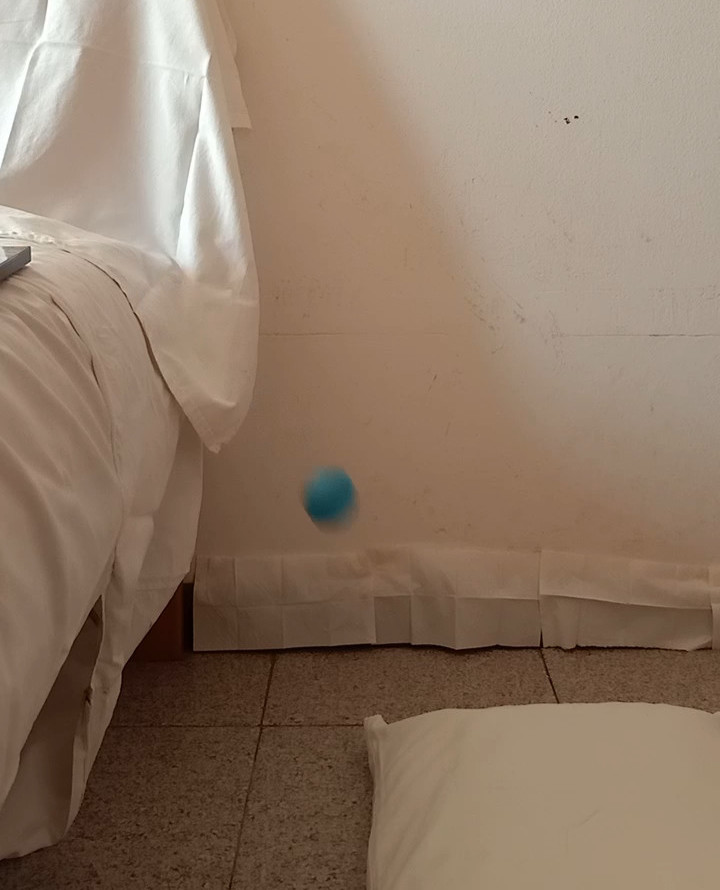
\includegraphics[width=0.60\textwidth]{setup_proiettile}
  \caption{L'apparato sperimentale per studiare il moto di un proiettile.}
  \label{fig:setup_proiettile}
\end{figure}

\section{Gli elementi del gioco}
Il gioco di modellamento richiede prima di tutto la scelta
dei suoi componenti: tabellone e pedine.

\subsection{Tabellone} 

\bibliography{bibliografia}{}
\bibliographystyle{plain}

\end{document}
